\documentclass[12pt, titlepage]{article}

\usepackage{fullpage}
\usepackage[round]{natbib}
\usepackage{multirow}
\usepackage{booktabs}
\usepackage{tabularx}
\usepackage{graphicx}
\usepackage{float}
\usepackage{hyperref}
\hypersetup{
    colorlinks,
    citecolor=blue,
    filecolor=black,
    linkcolor=red,
    urlcolor=blue
}
\usepackage{graphicx}
\graphicspath{ {./images/} }
\usepackage{caption}
\usepackage{enumitem}
\input{../../Comments}
%% Common Parts

\newcommand{\progname}{Chess Connect} % PUT YOUR PROGRAM NAME HERE
\newcommand{\authname}{Team \#4,
\\ Alexander Van Kralingen
\\ Arshdeep Aujla
\\ Jonathan Cels
\\ Joshua Chapman
\\ Rupinder Nagra} % AUTHOR NAMES without MacIDs 

\usepackage{hyperref}
    \hypersetup{colorlinks=true, linkcolor=blue, citecolor=blue, filecolor=blue,
                urlcolor=blue, unicode=false}
    \urlstyle{same}

\newcommand{\projectoverview}{

The Chess Connect project allows two users to play a game of chess on a physical board with the information being transmitted to an online web application over Bluetooth.
Currently, there is no way for players to seamlessly switch between playing on a physical board and playing online, but Chess Connect intends to change this by creating a central platform that will provide flexibility and remove barriers for new players looking to learn the game.

}

\newcounter{acnum}
\newcommand{\actheacnum}{AC\theacnum}
\newcommand{\acref}[1]{AC\ref{#1}}

\newcounter{ucnum}
\newcommand{\uctheucnum}{UC\theucnum}
\newcommand{\uref}[1]{UC\ref{#1}}

\newcounter{mnum}
\newcommand{\mthemnum}{M\themnum}
\newcommand{\mref}[1]{M\ref{#1}}

\begin{document}

\title{System Design for \progname} 
\author{\authname}
\date{\today}

\maketitle

\pagenumbering{roman}

\section{Revision History}

\begin{tabularx}{\textwidth}{p{3cm}p{2cm}X}
\toprule {\bf Date} & {\bf Version} & {\bf Notes}\\
\midrule
2023-01-11 & Arshdeep Aujla & Added Introduction, Purpose, User Interface, Other Considered Designs \\
2023-01-17 & Arshdeep Aujla & Added Hardware \\
\bottomrule
\end{tabularx}

\newpage

\section{Reference Material}

This section records information for easy reference.

\subsection{Abbreviations and Acronyms}

\renewcommand{\arraystretch}{1.2}
\begin{tabular}{l l} 
  \toprule		
  \textbf{symbol} & \textbf{description}\\
  \midrule 
  \progname & Explanation of program name\\
  \wss{...} & \wss{...}\\
  \bottomrule
\end{tabular}\\

\newpage

\tableofcontents

\newpage

\listoftables

\listoffigures

\newpage

\pagenumbering{arabic}

\section{Introduction}
This document outlines the system design portion of this project's design documentation. Design documentation 
is intended to separate the project into modular components to increase the project's understandability and reusability. \\
Other useful documents for this project are the following:
\begin{itemize}
  \item SRS
  \item HA
  \item VnV
\end{itemize}

\section{Purpose}
The purpose of this document is to outline a detailed system design. The system design includes system variables, user interfaces, a timeline for completion, and designs of many 
different components such as hardware, electrical componets, and communication protocols. This document also includes references to an intesive list of the project's
mechanical and electrical components and a reflection in the appendix. \\
Other documents relating to design are the following:
\begin{itemize}
  \item Software Architecture Document
  \item Detailed Design Document
\end{itemize}
\section{Scope}

\wss{Include a figure that show the System Context (showing the boundary between
your system and the environment around it.)}

\section{Project Overview}

\subsection{Normal Behaviour}

\subsection{Undesired Event Handling}

\wss{How you will approach undesired events}

\subsection{Component Diagram}

\subsection{Connection Between Requirements and Design} \label{SecConnection}

\wss{The intention of this section is to document decisions that are made
  ``between'' the requirements and the design.  To satisfy some requirements,
  design decisions need to be made.  Rather than make these decisions implicit,
  they are explicitly recorded here.  For instance, if a program has security
  requirements, a specific design decision may be made to satisfy those
  requirements with a password.}

\section{System Variables}

\wss{Include this section for Mechatronics projects}

\subsection{Monitored Variables}

\subsection{Controlled Variables}

\subsection{Constants Variables}

\section{User Interfaces}

\subsection*{Hardware Interface}
The user will interact with two main components of the hardware.
\begin{itemize}
  \item Magnetic chess pieces
  \item Physical chess board containing sensors
\end{itemize}
They will interact with the chess pieces and chess board as they would in a normal chess game. The chess board reflects a standard chess board, with 
LEDs in the center of each square. They would move the chess pieces on the board and remove them in according to the rules of chess. If the device
is set to beginner mode, the LEDs will light up in according to which available moves are available for that chess piece. They would interact with the LEDs
by using them as a guide for potential moves to make.

\subsection*{Software Interface}
The users will interact with the software component of this device through a web application. They would need a device with an internet connection and and internet browser
to view the application. The user will interact with this interface by visual viewing the chess board status in real time including a visualization of the chess piece locations.
They will also be able to turn on and off beginner mode in this interface through clicking an interactive button in the web application. 

\section{Design of Hardware}

\subsection*{Components Aquired}
Please refer to Appendix B for a detailed list of aquired mechanical components.

\subsection*{Finite State Machines}
Line 1 \\

Line2
\begin{figure}[h]
  \centering
  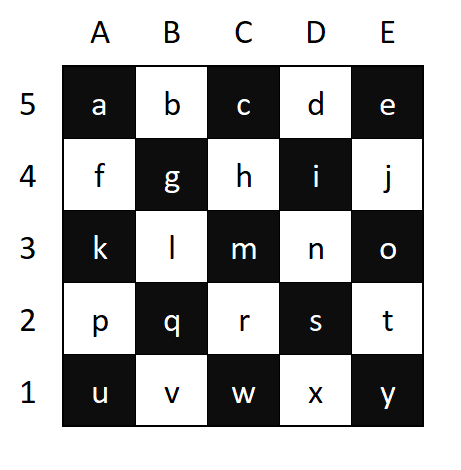
\includegraphics[width=0.5\textwidth]{line2}
  \caption{Caption}
\end{figure}

\begin{itemize}
  \item Case 1: King 
  \begin{minipage}{\linewidth}
    \centering
    
\includegraphics[width=0.5\textwidth]{king}
    \captionof{figure}{Transfer from R1 to R2 whenK1=1}
\end{minipage}
  \item Case 2: Queen   
  \begin{minipage}{\linewidth}
    \centering
    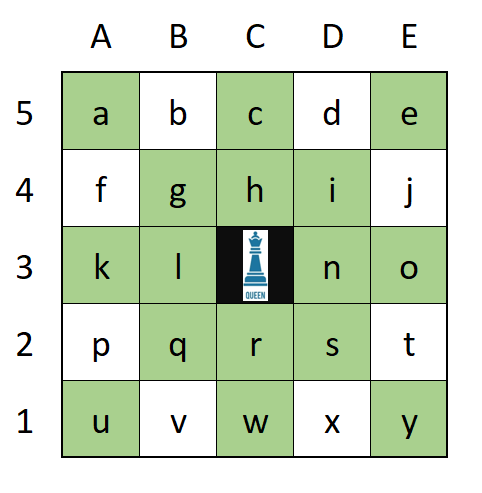
\includegraphics[width=0.5\textwidth]{queen}
    \captionof{figure}{Transfer from R1 to R2 whenK1=1}
\end{minipage}
  \item Case 3: Bishop   
  \begin{minipage}{\linewidth}
    \centering
    
\includegraphics[width=0.5\textwidth]{bishop}
    \captionof{figure}{Transfer from R1 to R2 whenK1=1}
\end{minipage}
  \item Case 4: Knight   
  \begin{minipage}{\linewidth}
    \centering
    
\includegraphics[width=0.5\textwidth]{knight}
    \captionof{figure}{Transfer from R1 to R2 whenK1=1}
\end{minipage}
  \item Case 5: Rook   
  \begin{minipage}{\linewidth}
    \centering
    
\includegraphics[width=0.5\textwidth]{rook}
    \captionof{figure}{Transfer from R1 to R2 whenK1=1}
\end{minipage}
  \item Case 6: Pawn   
  \begin{minipage}{\linewidth}
    \centering
    
\includegraphics[width=0.5\textwidth]{pawn}
    \captionof{figure}{Transfer from R1 to R2 whenK1=1}
\end{minipage}
\end{itemize}

\subsection*{Truth Table for LEDs}
\begin{figure}[h]
  \centering
  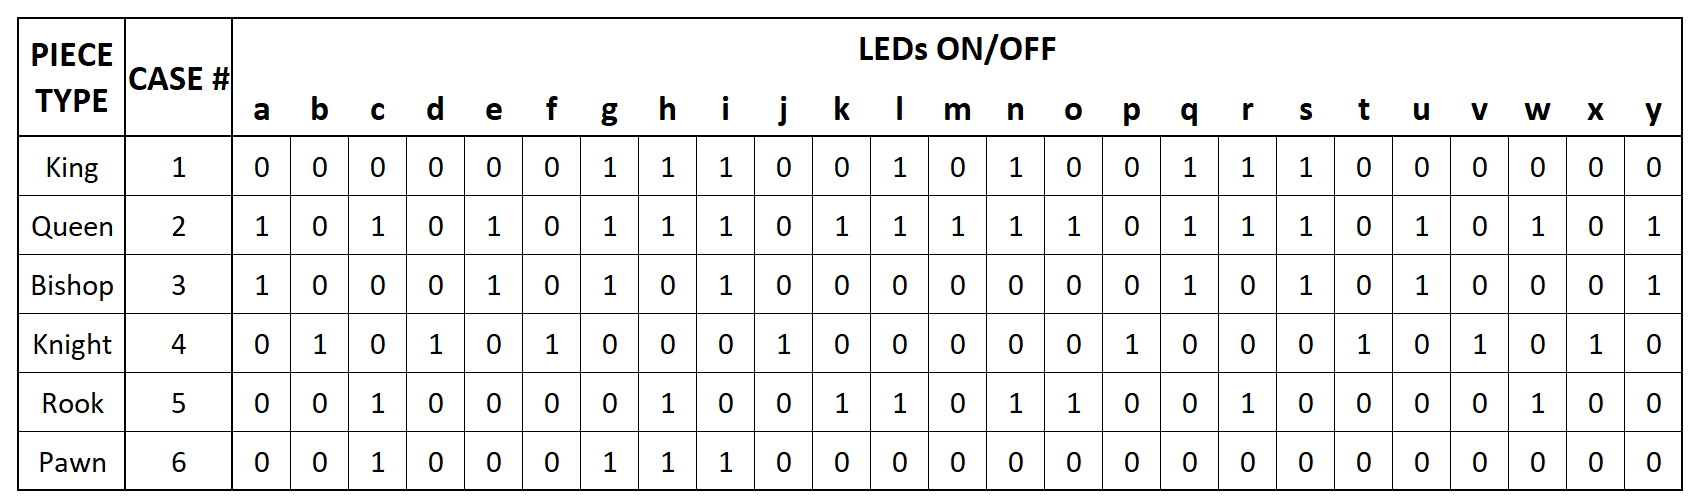
\includegraphics[width=1\textwidth]{truth_table}
  \caption{Caption}
\end{figure}

\subsection*{Deriving Boolean Expressions}
Line 3

\begin{enumerate}
  \item a =
  \item b =
  \item c =
  \item d =
  \item e =
  \item f =
  \item g =
  \item h =
  \item i =
  \item j =
  \item k =
  \item l =
  \item m =
  \item n =
  \item o =
  \item p =
  \item q =
  \item r =
  \item s =
  \item t =
  \item u =
  \item v =
  \item w =
  \item x =
  \item y =
\end{enumerate}

\section{Design of Electrical Components}
\subsection*{Aquired Components}
Please refer to Appendix C for a detailed list of aquired electrical components.

\wss{Most relevant for mechatronics projects}
\wss{Show what will be acquired}
\wss{Show what will be built, with detail on fabrication and materials}
\wss{Include appendices as appropriate, possibly with sketches, drawings,
circuit diagrams, etc}

\section{Design of Communication Protocols}

\wss{If appropriate}

\section{Timeline}

\wss{Schedule of tasks and who is responsible}

% \bibliographystyle {plainnat}
% \bibliography{../../../refs/References}

\newpage{}

\appendix

\section{Interface}

\wss{Include additional information related to the appearance of, and
interaction with, the user interface}

\section{Mechanical Hardware}
\begin{itemize}
  \item Arduino Mega
\end{itemize}

\section{Electrical Components}
\begin{itemize}
  \item 64 LEDs
  \item 64 1000ohm resistors
  \item 64 HALL sensors
  \item 64 1mF capacitors
  \item 3 breadboards
  \item 22 AND gate chips
  \item 300 pieces of wire
\end{itemize}

\section{Communication Protocols}

\section{Reflection}

\subsection*{Project Limitations}

\subsection*{Other Considered Designs}
One problem that we had to overcome in our design is that there are not enough input and output pins in one microcontoller for all of the components.
One solution we considered was having multiple microcontrollers for this project to ensure there is one input pin for each input sensor and one output pin for each output.
This design would be beneficial in the way of simplicity of code. The tradeoff would be the complexity in cordinating the communitcation between multiple microcontrollers and the 
web application. A second option to solve this problem is to use multiplexing to reduce the number of input and output pins needed for a large number of compnents. 
This option requires more complex code, but only requires one microcontroller device. We chose to implement the multiplexing option becasue it only used one device which saves money,
as well as eliminates the need to coordinate between multiple microcontrollers. 

The information in this section will be used to evaluate the team members on the
graduate attribute of Problem Analysis and Design.  Please answer the following questions:

\begin{enumerate}
  \item What are the limitations of your solution?  Put another way, given
  unlimited resources, what could you do to make the project better? (LO\_ProbSolutions)
  \item Give a brief overview of other design solutions you considered.  What
  are the benefits and tradeoffs of those other designs compared with the chosen
  design?  From all the potential options, why did you select documented design?
  (LO\_Explores)
\end{enumerate}

\end{document}